%\Lecture{Jayalal Sharma}{Sept 19, 2020}{07}{Catalan Bijections}{Anshu Yadav}{$\alpha$}{JS}

\subsection{Diagonal avoiding paths and Catlan numbers}
%Path coordinate Notation: 
In this section we explore the connection  between the above paths that we discussed and the Catalan number. 
Let us ask this question:
How many paths are there in the grid from $(0,0)$ to $(n,n)$ that avoids crossing the diagonal? 

We first define what \textit{crossing the diagonal} means. The diagonal consists of the points of the form $(i,i)$, $i\in\{0,\ldots, n\}$. A path $((u_0,v_0), \ldots, (u_{2n},v_{2n}))$ is said to be crossing the diagonal if it \textit{intersects} through the diagonal and goes to some point below the diagonal. Mathematically, a path is a diagonal crossing path if $\exists~i$ such that $u_i>v_i$. In particular, $\exists i: u_i = v_i+1$ (refer fig. \ref{fig:diagonal-crossing-path} for example. Any diagonal crossing path must necessarily pass through one of the red dots). Equivalently, in a diagonal avoiding path $\forall i\in\{0,\ldots, 2n\}, v_i\ge u_i$. A sample \emph{diagonal-avoiding path} is shown in the fig. \ref{fig:diagonal-avoiding-path} %\anote{explain $u_i = v_i+1$}
\begin{figure}[h!]
    \centering
    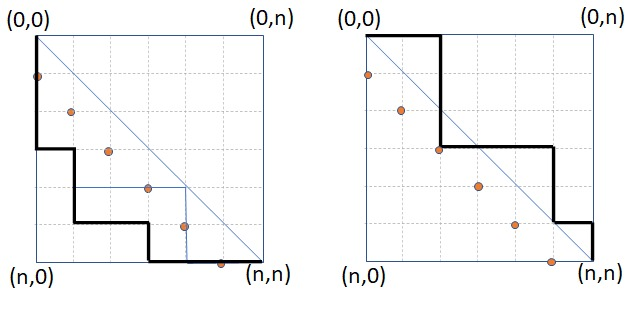
\includegraphics[width=0.7\linewidth]{diagonal-crossing.jpeg}
    \caption{Diagonal crossing paths. Note that path in (a) is crossing the diagonal at $(0,0)$}
    \label{fig:diagonal-crossing-path}
\end{figure}

\begin{figure}[h!]
    \centering
    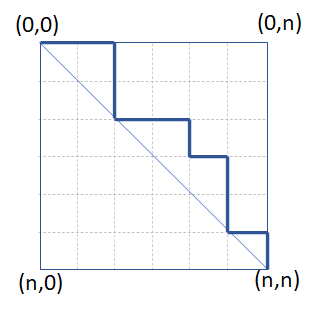
\includegraphics[width=0.4\linewidth]{diagonal-avoiding-path.png}
    \caption{A diagonal avoiding path. Observe that it can still touch the diagonal}
    \label{fig:diagonal-avoiding-path}
\end{figure}

Before computing this number, an obvious question is what is the connection between such restricted paths and Catalan number. It turns out that the set of diagonal avoiding paths from $(0,0)$ to $(n,n)$ is in bijection with the set of balanced paranthesized strings of length $2n$. Hence, to count the number of balanced paranthesized strings of length $2n$, which is also the Catalan number, we only need to count the diagonal avoiding paths from $(0,0)$ to $(n,n)$. Let us first establish the bijection between the two.

\subsection{Bijection from Diagonal avoiding paths to Balanced parenthesisation problem}
Intuitively, the bijection can be defined as follows: for any given balanced parenthesized string $w = w_1w_2\ldots w_{2n}$, the corresponding path from $(0,0)$ to $(n,n)$ is obtained by starting from position $(0,0)$, and scanning the string from left to right. Take  right move whenever $`('$ is encountered and a down move for $`)'$. Formally we define the bijection as follows:
\medskip{}

\noindent\underline{Defining the bijection:} Let $P$ be the set of diagonal avoiding paths from $(0,0)$ to $(n,n)$  and $B$ be the set of balanced paranthesized  strings of length $2n$ over the alphabets $\{(,)\}$. Define the bijection $\phi:B\rightarrow P$ as follows:\\
For $w=w_1 w_2 \ldots w_{2n}\in B$, $\phi(w) = (u_0,v_0), (u_1,v_1), \ldots, (u_i, v_i), \ldots, (u_{2n}, v_{2n})$, where 
\begin{enumerate}
    \item $(u_0,v_0)=(0,0)$ 
    \item $\forall i\in\{1,2,\ldots, 2n\}$\\
    \[
    (u_i, v_i) = 
    \begin{cases}  
    (u_{i-1}+1, v_{i-1})& ~~~~\text{if }w_i=)\\
    (u_{i-1}, v_{i-1}+1)&~~~~\text{if }w_i=(
    \end{cases}
    \]
    % $(u_i, v_i) = (u_{i-1}+1, v_{i-1})~~~~\text{if }w_i='('$\\
    % $(u_i, v_i) = (u_{i-1}, v_{i-1}+1)~~~~\text{if }w_i=')'$
\end{enumerate}
\underline{Proof of bijection}
\begin{description}
\item \textit{Well-defined:} From the above description, given any string $w$, $\phi(w)$ is uniquely defined. Further, for any string $w\in B$, since the number of $'('$ is same as  the number of $')' = n$, the corresponding path has $n$ right and $n$ down moves and hence it ends at $(n,n)$. Also, since the number of left brackets is greater than or equal to the number of right brackets in any prefix of $w$, for all $i\in[2n]$, $v_i\ge u_i$. This shows that $\forall w\in B, \phi(w)\in P$. Hence,  $\phi$ is well-defined.
\item \textit{Injective:} Let $w, w'$ be two different strings in set $B$. Then $\exists~$ an index $i\in[2n]$ where $w_i\ne w'_i$. Hence $\phi(w)$ and $\phi(w')$ also differ at the $i$th step, where one of the paths takes one step right while the other takes one step down. 
\item \textit{Surjective:} 
Given any path $((0,0), (u_1, v_1), \ldots, (u_{2n}, v_{2n}))$ the corresponding string $w\in B$ is defined as follows:\\
$\forall i\in[2n]$
\[
w_i = 
\begin{cases}
`(`& ~~~~~\text{if } (u_i, v_i) = (u_{i-1}, v_{i-1}+1)\\
`)`& ~~~~~\text{if } (u_i,v_i) = (u_{i-1}+1, v_{i-1})
\end{cases}
\]
We can verify that the string $w$ indeed is in set $B$, because firstly, for any path in $P$, $\forall i, v_i\ge u_i$ and hence by definition, number of left brackets $`(`$ in $w$ is greater than or equal to number of right brackets, $`(`$ in any prefix of $w$. Secondly, for any path to reach from $(0,0)$ to $(n,n)$ it must have $n$ right moves (increase in 2nd coordinate) and $n$ down moves (increase in 1st coordinate) and hence $w$ must have $n$ left brackets and $n$ right brackets.
\end{description}


% Properties:
% %$\phi(w_1)=u_1$ and $\phi(w_2)=u_2$ will be same till $(i-1)$th step, i.e. $(u_{1,(i-1)}, v_{1,(i-1)}=(u_{2,(i-1)}, v_{2,(i-1)}$ for $j=0$ to $i-1$.

\subsection{Counting the number of diagonal avoiding paths} 
Having established the bijection between Catalan number and diagonal avoiding paths, we get  
\begin{equation}
\label{eq:catalan-expr-1}
    C_n = \# \text{ of diagonal avoiding paths from } (0,0) to (n,n) 
\end{equation}
So, our next task is to count the number of diagonal avoiding paths from $(0,0)$ to $(n,n)$. 
To count this, we take following approach. Let us call the diagonal avoiding paths as \textit{good} paths and diagonal crossing paths as \textit{bad} paths. Then,
\begin{equation}
\label{eq:no-of-good-paths}
\Large
    \substack{\text{\# of diagonal avoiding paths }\\ \text{from } (0,0) \text{ to } (n,n)}  = \substack{\text{\# of paths }\\ \text{from } (0,0) \text{ to } (n,n)} - \substack{\text{\# of diagonal crossing paths }\\ \text{from } (0,0) \text{ to } (n,n)}
\end{equation}  

So, now our revised goal is to count the number of diagonal crossing paths from $(0,0)$ to $(n,n)$. How do we do that? Here again bijection plays an important role. The idea is to translate diagonal crossing paths into  different kind of paths which are easy to count. 

Let us define the following path translation:  Let $\pi=(0,0), (u_1,v_1), \ldots, (u_{2n}, v_{2n})$ be  a diagonal crossing path. Then there must exist $i$ such that $u_i = v_i+1$. There can be many such indices as the path can cross the diagonal multiple times. Choose $i$ to be the least such index. Let $u_i = \ell$, then the first co-ordinate after crossing the diagonal is $(\ell, \ell-1)$. Let us call this point $P$ (refer fig. \ref{fig:reflecting-path}(a)). Then to find the translated path we reflect the part of the path $\pi$ after point $P$ w.r.t. the main diagonal. 

\begin{figure}[h!]
    \centering
    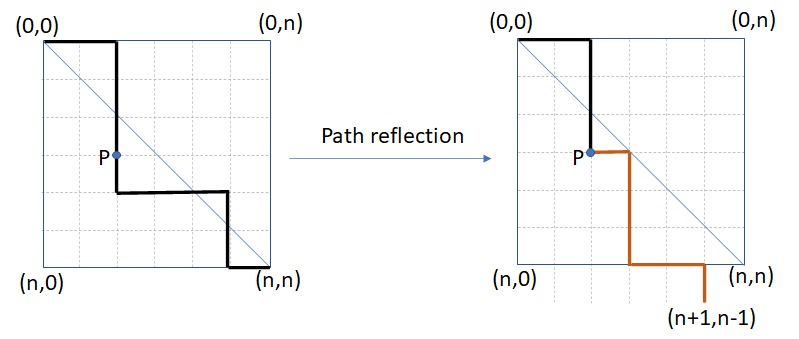
\includegraphics[width=0.7\linewidth]{reflecting-path.jpeg}
    \caption{Point P in a diagonal crossing path and the reflected path after P}
    \label{fig:reflecting-path}
\end{figure}

More precisely, we can divide the diagonal crossing path into two stretch $S_1, S_2$, where $S_1$ is the part of the path between $(0,0)$ to $P$ and $S_2$ is the part of the path between $P$  to $(n,n)$. 
Then to translate $\pi$ into a new path, replace $S_2$ with $S_2'$  to get a new path $\pi' = S_1S_2'$. The replacement $S_2'$ is defined as follows:
\begin{itemize}
    \item[-] replace downward edges with right edges and 
    \item[-] replace right edges with downward edges.
\end{itemize} Refer fig. \ref{fig:reflecting-path}(b)
We can observe that the new path $\pi'$ described in this way is always between $(0,0)$ to $(n+1, n-1)$. The argument for this goes as follows:

Originally (in $S_2$), $(\ell, \ell-1)$ goes to $(n,n)$ which means it takes $(n-\ell)$ downward moves and $(n-\ell+1)$ right moves. Since, we are swapping the right and downward moves to get $S_2'$ from $S_2$, there are $(n-\ell+1)$ downward moves and $(n-\ell)$ right moves from point $P=(\ell, \ell-1)$ in $S_2'$. Thus, $S_2'$ goes from $(\ell, \ell-1)$ to $(\ell+n-\ell+1, \ell-1+n-\ell) = (n+1, n-1)$ and hence, $\pi' = S_1S_2'$ is a path from $(0,0)$ to $(n+1, n-1)$. 

Thus we have established that any diagonal crossing path from $(0,0)$ to $(n,n)$ maps to a path from $(0,0)$ to $(n+1,n-1)$ after applying the transformation described above. The converse is also true, i.e., given any path from $(0,0)$ to $(n+1, n-1)$, we can translate it back to a diagonal crossing path from $(0,0)$ to $(n,n)$ by using the same reflection technique.  Thus, we get a bijection between the set of diagonal crossing paths from $(0,0)$ to $(n,n)$ to the set of paths from $(0,0)$ to $(n+1,n-1)$. We formally define the translation and prove that it is indeed a bijection.
\begin{description}
\item \underline{Bijection:}
Let $A$ be the set of diagonal crossing paths from $(0,0)$ to $(n,n)$ and $B$ be the set of paths from $(0,0)$ to $(n+1,n-1)$. Then the mapping $\phi:A\rightarrow B$ is formally defined as follows: 
\\
Let $\pi=(0,0), (u_1,v_1), \ldots, (u_{2n}, v_{2n})$ and $(u_i, v_i)$ be the first point when $\pi$ crosses the diagonal. Then $\phi(\pi) = \pi'=(0,0), (u'_1,v'_1), \ldots, (u'_{2n}, v'_{2n})$ is given by:
\begin{enumerate}
    \item $\forall 1\le j\le i, (u'_j, v'_j) = (u_j, v_j)$
    \item $\forall i+1\le j\le 2n$, 
    \[
    (u'_j, v'_j) = 
    \begin{cases}
    (u'_{j-1}+1, v'_{j-1})& ~~~~~\text{if } (u_j, v_j) = (u_{j-1}, v'_{j-1}+1)\\
    (u'_{j-1}, v'_{j-1}+1)& ~~~~~\text{if } (u_j, v_j) = (u_{j-1}+1, v'_{j-1})
    \end{cases}
    \]
\end{enumerate}
% We can verify that $\phi:A\rightarrow B$ satisfies all the properties of a bijection as follows:
\item \textit{Well-defined:} We already observed that any path $\pi\in A$ from $(0,0)$ to $(n,n)$ maps to a path $(0,0)$ to $(n+1,n-1)$. Hence $\phi$ is well defined.
\item \textit{Injection:} Consider two different diagonal crossing paths $\pi_1$ and $\pi_2$. Let $\pi_1 = S_{1,1}S_{1,2}$ and $\pi_2 = S_{2,1}S_{2,2}$, where the two components $S_{i,1}$ and $S_{i,2}$ for $i\in\{1,2\}$ are as defined before. Then following two cases are possible:
\begin{itemize}
    \item Case1: $S_{11}\ne S_{21}$. Then $\pi_1'\ne \pi_2'$, because the first component is copied as it is in the translation, i.e. $\pi_1' = S_{1,1}S_{1,2}'$ and $\pi_2' = S_{2,1}S_{2,2}'$.
    \item Case2: $S_{11}= S_{21}$, but $S_{12}\ne S_{22}$. In this case $S_{12}'\ne S_{22}'$ because of the way it is defined, i.e. for every right move there is a downwards move and vice-versa. Hence, $\pi_i'\ne \pi_2'$.
\end{itemize}
\item \textit{Surjective:} Given any path $\pi'$ from  $(0,0)$ to $(n+1,n-1)$, we can construct the corresponding path $\pi$ from $(0,0)$ to $(n,n)$, such that $\phi(\pi) = \pi'$, as follows.\\
Let $\pi'=(0,0), (u'_1,v'_1), \ldots, (u'_{2n}, v'_{2n})$. Since $\pi'$ goes to $(n+1, n-1)$ which is below the diagonal there must exist $i$ such that $(u'_i,v'_i)$ is below the diagonal. Again, there can be many such indices. Take $i$ to be the first such index. Same as before, let $\pi' = S_1'S_2'$, where $S_1'$ is the path from $(0,0)$ to $(u_i', v_i')$ and  $S_1'$ is the path from $(u_i',v_i')$ to $(u_{2n}', v_{2n}')$. Then $\pi = S_1'S_2$ where $S_2$ is obtained from $S_2'$ by swapping the right and downwards moves. Mathematically, let $\pi=(0,0), (u_1,v_1), \ldots, (u_{2n}, v_{2n})$. Then
\begin{enumerate}
    \item $\forall j\le i$, $(u_j, v_j) = (u_j', v_j')$
    \item $\forall~i+1\le j\le 2n$
    \[
    (u_j, v_j) =
    \begin{cases}
    (u_{j-1}+1, v_{j-1}) & ~~~~~\text{if } (u_j', v_j') = (u_{j-1}', v_{j-1}'+1)\\
    (u_{j-1}, v_{j-1}+1) & ~~~~~\text{if } (u_j', v_j') = (u_{j-1}'+1, v_{j-1}')
    \end{cases}
    \]
\end{enumerate}
Again by the same argument as before it can be verified that $\pi$ is a diagonal crossing path from $(0,0)$ to $(n,n)$. We write it here for completeness. Let $(\ell, \ell-1)$ be the first point when $\pi'$ crosses the diagonal. Then since the path from $(0,0)$ to $(\ell, \ell-1)$ remains as it is in $\pi$, it is a diagonal crossing path. Further since $\pi'$ is path from $(0,0)$ to $(n+1, n-1)$, it takes $n+1-\ell$ downward steps and $n-\ell$ right steps from $(\ell, \ell-1)$. Hence, $\pi$ takes $n+1-\ell$ right and $n-\ell$ downward steps from $(\ell, \ell-1)$. Thus, $\pi$ ends at $(\ell+n-\ell, \ell-1+n+1-\ell) = (n,n)$. 
\end{description}

Thus, we have established a bijection between the set of diagonal crossing paths from $(0,0)$ to $(n,n)$ and the set of  paths from $(0,0)$ to $(n+1,n-1)$. Hence, 
\begin{eqnarray*}
    \# \text{of diagonal crossing paths from } (0,0) \text{ to } (n,n) &=& \# \text{of paths from } (0,0) \text{ to } (n+1,n-1)\\
    &= &{2n\choose n+1}
\end{eqnarray*}
Hence, from~\eqref{eq:catalan-expr-1},\eqref{eq:no-of-good-paths},
\begin{align*} %\label{eq:no-of-good-paths-2}
C_n &= \# \text{of diagonal avoiding paths from} (0,0) \text{ to } (n,n)\\
%\Large
 %   \substack{\text{\# of diagonal avoiding paths }\\ \text{from } (0,0) \text{ to } (n,n)} 
     &= \Large \substack{\text{\# of paths }\\ \text{from } (0,0) \text{ to } (n,n)} - \Large\substack{\text{\# of diagonal crossing paths }\\ \text{from } (0,0) \text{ to } (n,n)}\\
    &= {2n\choose n} - {2n\choose n+1}\\
    & = {2n\choose n} - \frac{n}{n+1}{2n\choose n}\\
    &=\frac{1}{n+1}{2n\choose n}
\end{align*}  

Here, in the second last line, we have used the identity: $${2n\choose n+1} = \frac{n}{n+1}{2n\choose n}.$$









% Let us define the following path translation: Let $p=(0,0), (u_1,v_1), \ldots, (u_{2n}, v_{2n})$ be  a diagonal crossing path which goes below the diagonal at point $(u_i, v_i)$ for for the first time. Then, translate the path $p$ to a new path $p' = (u'_0, v'_0), (u'_1,v'_1), \ldots, (u'_{2n}, v'_{2n})$ by \textit{reflexing} $p$ between  $(u_i, v_i)$ and $(u_{2n}, v_{2n})$ in the sense that whenever $p$ goes right, $p'$ goes down, and whenever $p$ goes down, $p'$ moves right. Mathematically,
% \begin{enumerate}
%     \item $\forall 1\le j\le i, (u'_j, v'_j) = (u_j, v_j)$
%     \item $\forall i+1\le j\le 2n$, 
%     \[
%     (u'_j, v'_j) = 
%     \begin{cases}
%     (u'_{j-1}+1, v'_{j-1})& ~~~~~\text{if } (u_j, v_j) = (u_{j-1}, v'_{j-1}+1)\\
%     (u'_{j-1}, v'_{j-1}+1)& ~~~~~\text{if } (u_j, v_j) = (u_{j-1}+1, v'_{j-1})
%     \end{cases}
%     \]
% \end{enumerate}
% In the example, we can see that the translated path ends up at $(n+1, n-1)$. In general, we can prove the following: The above defined translation of any diagonal crossing path $p$ from $(0,0)$ to $(n,n)$ always ends at $(n+1, n-1)$.
% \begin{proof}
% Let $p$ croses the diagonal for the first time at $(u_i, v_i)$. Then 
% $$u_i = v_i+1.$$ 
% From $(u_i, v_i)$, $p$ moves $(n-u_i)$ steps down and $(n-v_i)$ steps in the right to reach $(n,n)$. Hence, the translated path $p'$ takes $(n-u_i)$ steps right and $(n-v_i)$ steps down from $(u_i, v_i)$ and ends at $$ (u_i+n-v_i, v_i+n-u_i) = (n+(u_i-v_i), n+(v_i-u_i)) = (n+1, n-1)$$. 
% \end{proof}

% Conversely, any path $p'$ from $(0,0)$ to $(n+1, n-1)$ can be mapped to a diagonal crossing path from $(0,0)$ to $(n,n)$. Intuitively, this can be done by again reflecting it  from the point $(u_i, v_i)$, where it crosses the diagonal for the first time. Note that such a point always exist because to reach the point $(n+1, n-1)$ $p'$ must cross the diagonal because $(n+1, n-1)$ is below the diagonal. Using the same argument as above, it can be shown that this translates $p'$ into a diagonal crossing path from $(0,0)$ to $(n,n)$.

% Thus, we get a bijection between the set of diagonal crossing paths from $(0,0)$ to $(n,n)$ and the set of paths from $(0,0)$ to $(n+1,n-1)$ defined formally as follows:\\

% Definition: Let $A$ be the set of diagonal crossing paths from $(0,0)$ to $(n,n)$ and $B$ be the set of paths from $(0,0)$ to $(n+1,n-1)$. Then a bijection $\phi:A\rightarrow B$ is defined as follows:

% For any path $p = (u_0, v_0), (u_1, v_1), \ldots, (u_{2n}, v_{2n})\in A$, let $(u_i, v_i)$ be the point where the path crosses the diagonal for the first time. That is, 
% \begin{enumerate}
%     \item $\forall j<i, v_j\ge u_j$, and
%     \item $u_i=v_i+1$
% \end{enumerate}
% Then $\phi(p)=p' = (u'_0, v'_0), (u'_1, v'_1), \ldots, (u'_{2n}, v'_{2n})$, where
% \begin{enumerate}
%     \item 
% \end{enumerate}
\begin{ex}
\item Try to establish a bijection between the set of different possible polygon triangulation in a polygon of $n+2$ nodes and the set of binary trees with $n$ internal nodes.

\textit{Hint: associate each internal node with a triangle in a triangulation. Then, each internal node will have degree three, which is the case for full binary tree, except for the leaves. Leaves will correspond to those triangles whose one of the edge is the boundary of the polygon.}
\end{ex}

 

